\documentclass[11pt,bibliography=totocnumbered]{scrartcl}
\usepackage[usenames,dvipsnames]{xcolor}
\usepackage[utf8]{inputenc}
\usepackage[T1]{fontenc}
\usepackage{fontspec-luatex}
\usepackage{amsmath,amssymb,amstext}
\usepackage{graphicx}
\usepackage[automark]{scrpage2}
\usepackage{url}
\usepackage[style=numeric-verb,backend=bibtex8,sorting=none, maxbibnames=99]{biblatex}
\usepackage[nottoc,numbib,notlof]{tocbibind}
\usepackage[ngerman]{babel}
\usepackage{titlesec}
\usepackage{tocloft}
\usepackage[bottom=1.5in]{geometry}
\usepackage{tikz}
\usepackage{pgfplots}
\usepackage[colorlinks=true,urlcolor=blue,linkcolor=Sepia,citecolor=Sepia,unicode,breaklinks=true,backref=true]{hyperref}
\usepackage[onehalfspacing]{setspace}
\usepackage{float}
\usepackage[parfill]{parskip}
\usepackage[utf8]{inputenc}
\usepackage{listings}
\usepackage{listings}
\usepackage{amsmath}
\usepackage{mathtools}
\usepackage{xpatch}
\usepackage[xindy, nopostdot, nonumberlist]{glossaries}

\newcommand{\listequationsname}{Formelverzeichnis}
\newlistof{myequations}{equ}{\listequationsname}
\newcommand{\myequations}[1]{%
\addcontentsline{equ}{myequations}{\protect\numberline{\theequation}#1}}
\addtolength{\cftmyequationsnumwidth}{12pt}

\colorlet{punct}{red!60!black}
\definecolor{background}{HTML}{EEEEEE}
\definecolor{delim}{RGB}{20,105,176}
\colorlet{numb}{magenta!60!black}

\definecolor{maroon}{cmyk}{0, 0.87, 0.68, 0.32}
\definecolor{halfgray}{gray}{0.55}
\definecolor{ipython_frame}{RGB}{207, 207, 207}
\definecolor{ipython_bg}{RGB}{247, 247, 247}
\definecolor{ipython_red}{RGB}{186, 33, 33}
\definecolor{ipython_green}{RGB}{0, 128, 0}
\definecolor{ipython_cyan}{RGB}{64, 128, 128}
\definecolor{ipython_purple}{RGB}{170, 34, 255}

\lstset{
	breaklines=true,
	extendedchars=true,
	literate=
	{á}{{\'a}}1 {é}{{\'e}}1 {í}{{\'i}}1 {ó}{{\'o}}1 {ú}{{\'u}}1
	{Á}{{\'A}}1 {É}{{\'E}}1 {Í}{{\'I}}1 {Ó}{{\'O}}1 {Ú}{{\'U}}1
	{à}{{\`a}}1 {è}{{\`e}}1 {ì}{{\`i}}1 {ò}{{\`o}}1 {ù}{{\`u}}1
	{À}{{\`A}}1 {È}{{\'E}}1 {Ì}{{\`I}}1 {Ò}{{\`O}}1 {Ù}{{\`U}}1
	{ä}{{\"a}}1 {ë}{{\"e}}1 {ï}{{\"i}}1 {ö}{{\"o}}1 {ü}{{\"u}}1
	{Ä}{{\"A}}1 {Ë}{{\"E}}1 {Ï}{{\"I}}1 {Ö}{{\"O}}1 {Ü}{{\"U}}1
	{â}{{\^a}}1 {ê}{{\^e}}1 {î}{{\^i}}1 {ô}{{\^o}}1 {û}{{\^u}}1
	{Â}{{\^A}}1 {Ê}{{\^E}}1 {Î}{{\^I}}1 {Ô}{{\^O}}1 {Û}{{\^U}}1
	{œ}{{\oe}}1 {Œ}{{\OE}}1 {æ}{{\ae}}1 {Æ}{{\AE}}1 {ß}{{\ss}}1
	{ç}{{\c c}}1 {Ç}{{\c C}}1 {ø}{{\o}}1 {å}{{\r a}}1 {Å}{{\r A}}1
	{€}{{\EUR}}1 {£}{{\pounds}}1
}

\lstdefinelanguage{pythoninline}{
	morekeywords={access,and,break,class,continue,def,del,elif,else,except,exec,finally,for,from,global,if,import,in,is,lambda,not,or,pass,print,raise,return,try,while},
	morekeywords=[2]{abs,all,any,basestring,bin,bool,bytearray,callable,chr,classmethod,cmp,compile,complex,delattr,dict,dir,divmod,enumerate,eval,execfile,filter,float,format,frozenset,getattr,globals,hasattr,hash,help,hex,id,input,int,isinstance,issubclass,iter,len,list,locals,long,map,max,memoryview,min,next,object,oct,open,ord,pow,property,range,raw_input,reduce,reload,repr,reversed,round,set,setattr,slice,sorted,staticmethod,str,sum,super,tuple,type,unichr,unicode,vars,xrange,zip,apply,buffer,coerce,intern},
	sensitive=true,
	morecomment=[l]\#,
	morestring=[b]',
	morestring=[b]",
	morestring=[s]{'''}{'''},
	morestring=[s]{"""}{"""},
	morestring=[s]{r'}{'},
	morestring=[s]{r"}{"},
	morestring=[s]{r'''}{'''},
	morestring=[s]{r"""}{"""},
	morestring=[s]{u'}{'},
	morestring=[s]{u"}{"},
	morestring=[s]{u'''}{'''},
	morestring=[s]{u"""}{"""},
	% {replace}{replacement}{lenght of replace}
	% *{-}{-}{1} will not replace in comments and so on
	literate=
	{á}{{\'a}}1 {é}{{\'e}}1 {í}{{\'i}}1 {ó}{{\'o}}1 {ú}{{\'u}}1
	{Á}{{\'A}}1 {É}{{\'E}}1 {Í}{{\'I}}1 {Ó}{{\'O}}1 {Ú}{{\'U}}1
	{à}{{\`a}}1 {è}{{\`e}}1 {ì}{{\`i}}1 {ò}{{\`o}}1 {ù}{{\`u}}1
	{À}{{\`A}}1 {È}{{\'E}}1 {Ì}{{\`I}}1 {Ò}{{\`O}}1 {Ù}{{\`U}}1
	{ä}{{\"a}}1 {ë}{{\"e}}1 {ï}{{\"i}}1 {ö}{{\"o}}1 {ü}{{\"u}}1
	{Ä}{{\"A}}1 {Ë}{{\"E}}1 {Ï}{{\"I}}1 {Ö}{{\"O}}1 {Ü}{{\"U}}1
	{â}{{\^a}}1 {ê}{{\^e}}1 {î}{{\^i}}1 {ô}{{\^o}}1 {û}{{\^u}}1
	{Â}{{\^A}}1 {Ê}{{\^E}}1 {Î}{{\^I}}1 {Ô}{{\^O}}1 {Û}{{\^U}}1
	{œ}{{\oe}}1 {Œ}{{\OE}}1 {æ}{{\ae}}1 {Æ}{{\AE}}1 {ß}{{\ss}}1
	{ç}{{\c c}}1 {Ç}{{\c C}}1 {ø}{{\o}}1 {å}{{\r a}}1 {Å}{{\r A}}1
	{€}{{\EUR}}1 {£}{{\pounds}}1
	%
	{^}{{{\color{ipython_purple}\^{}}}}1
	{=}{{{\color{ipython_purple}=}}}1
	%
	{+}{{{\color{ipython_purple}+}}}1
	{*}{{{\color{ipython_purple}$^\ast$}}}1
	{/}{{{\color{ipython_purple}/}}}1
	%
	{+=}{{{+=}}}1
	{-=}{{{-=}}}1
	{*=}{{{$^\ast$=}}}1
	{/=}{{{/=}}}1,
	literate=
	*{-}{{{\color{ipython_purple}-}}}1
	{?}{{{\color{ipython_purple}?}}}1,
	%
	identifierstyle=\color{black}\ttfamily,
	commentstyle=\color{ipython_cyan}\ttfamily,
	stringstyle=\color{ipython_red}\ttfamily,
	keepspaces=true,
	showspaces=false,
	showstringspaces=false,
	rulecolor=\color{ipython_frame},
	frame=single,
	frameround={t}{t}{t}{t},
	framexleftmargin=6mm,
	numbers=left,
	numberstyle=\tiny\color{halfgray},
	backgroundcolor=\color{ipython_bg},
	% extendedchars=true,
	basicstyle=\fontsize{13}{15}\selectfont\ttfamily,
	keywordstyle=\color{ipython_green}\ttfamily,
	tabsize=2
}

\lstdefinelanguage{python}{
	morekeywords={access,and,break,class,continue,def,del,elif,else,except,exec,finally,for,from,global,if,import,in,is,lambda,not,or,pass,print,raise,return,try,while},
	morekeywords=[2]{abs,all,any,basestring,bin,bool,bytearray,callable,chr,classmethod,cmp,compile,complex,delattr,dict,dir,divmod,enumerate,eval,execfile,filter,float,format,frozenset,getattr,globals,hasattr,hash,help,hex,id,input,int,isinstance,issubclass,iter,len,list,locals,long,map,max,memoryview,min,next,object,oct,open,ord,pow,property,range,raw_input,reduce,reload,repr,reversed,round,set,setattr,slice,sorted,staticmethod,str,sum,super,tuple,type,unichr,unicode,vars,xrange,zip,apply,buffer,coerce,intern},
	sensitive=true,
	morecomment=[l]\#,
	morestring=[b]',
	morestring=[b]",
	morestring=[s]{'''}{'''},
	morestring=[s]{"""}{"""},
	morestring=[s]{r'}{'},
	morestring=[s]{r"}{"},
	morestring=[s]{r'''}{'''},
	morestring=[s]{r"""}{"""},
	morestring=[s]{u'}{'},
	morestring=[s]{u"}{"},
	morestring=[s]{u'''}{'''},
	morestring=[s]{u"""}{"""},
	% {replace}{replacement}{lenght of replace}
	% *{-}{-}{1} will not replace in comments and so on
	literate=
	{á}{{\'a}}1 {é}{{\'e}}1 {í}{{\'i}}1 {ó}{{\'o}}1 {ú}{{\'u}}1
	{Á}{{\'A}}1 {É}{{\'E}}1 {Í}{{\'I}}1 {Ó}{{\'O}}1 {Ú}{{\'U}}1
	{à}{{\`a}}1 {è}{{\`e}}1 {ì}{{\`i}}1 {ò}{{\`o}}1 {ù}{{\`u}}1
	{À}{{\`A}}1 {È}{{\'E}}1 {Ì}{{\`I}}1 {Ò}{{\`O}}1 {Ù}{{\`U}}1
	{ä}{{\"a}}1 {ë}{{\"e}}1 {ï}{{\"i}}1 {ö}{{\"o}}1 {ü}{{\"u}}1
	{Ä}{{\"A}}1 {Ë}{{\"E}}1 {Ï}{{\"I}}1 {Ö}{{\"O}}1 {Ü}{{\"U}}1
	{â}{{\^a}}1 {ê}{{\^e}}1 {î}{{\^i}}1 {ô}{{\^o}}1 {û}{{\^u}}1
	{Â}{{\^A}}1 {Ê}{{\^E}}1 {Î}{{\^I}}1 {Ô}{{\^O}}1 {Û}{{\^U}}1
	{œ}{{\oe}}1 {Œ}{{\OE}}1 {æ}{{\ae}}1 {Æ}{{\AE}}1 {ß}{{\ss}}1
	{ç}{{\c c}}1 {Ç}{{\c C}}1 {ø}{{\o}}1 {å}{{\r a}}1 {Å}{{\r A}}1
	{€}{{\EUR}}1 {£}{{\pounds}}1
	%
	{^}{{{\color{ipython_purple}\^{}}}}1
	{=}{{{\color{ipython_purple}=}}}1
	%
	{+}{{{\color{ipython_purple}+}}}1
	{*}{{{\color{ipython_purple}$^\ast$}}}1
	{/}{{{\color{ipython_purple}/}}}1
	%
	{+=}{{{+=}}}1
	{-=}{{{-=}}}1
	{*=}{{{$^\ast$=}}}1
	{/=}{{{/=}}}1,
	literate=
	*{-}{{{\color{ipython_purple}-}}}1
	{?}{{{\color{ipython_purple}?}}}1,
	%
	identifierstyle=\color{black}\ttfamily,
	commentstyle=\color{ipython_cyan}\ttfamily,
	stringstyle=\color{ipython_red}\ttfamily,
	keepspaces=true,
	showspaces=false,
	showstringspaces=false,
	rulecolor=\color{ipython_frame},
	frame=single,
	frameround={t}{t}{t}{t},
	framexleftmargin=6mm,
	numbers=left,
	numberstyle=\tiny\color{halfgray},
	backgroundcolor=\color{ipython_bg},
	% extendedchars=true,
	basicstyle=\fontsize{10}{12}\selectfont\ttfamily,
	keywordstyle=\color{ipython_green}\ttfamily,
	tabsize=2
}

\lstdefinelanguage{json}{
	basicstyle=\normalfont\ttfamily,
	numbers=left,
	numberstyle=\scriptsize,
	stepnumber=1,
	numbersep=8pt,
	showstringspaces=false,
	breaklines=true,
	tabsize=2,
	frame=lines,
	backgroundcolor=\color{background},
	literate=
	*{0}{{{\color{numb}0}}}{1}
	{1}{{{\color{numb}1}}}{1}
	{2}{{{\color{numb}2}}}{1}
	{3}{{{\color{numb}3}}}{1}
	{4}{{{\color{numb}4}}}{1}
	{5}{{{\color{numb}5}}}{1}
	{6}{{{\color{numb}6}}}{1}
	{7}{{{\color{numb}7}}}{1}
	{8}{{{\color{numb}8}}}{1}
	{9}{{{\color{numb}9}}}{1}
	{:}{{{\color{punct}{:}}}}{1}
	{,}{{{\color{punct}{,}}}}{1}
	{\{}{{{\color{delim}{\{}}}}{1}
	{\}}{{{\color{delim}{\}}}}}{1}
	{[}{{{\color{delim}{[}}}}{1}
	{]}{{{\color{delim}{]}}}}{1},
}



\addbibresource{Quellen.bib}
\nocite{*}

\title{Automatische Analyse von Stimmmerkmalen zur Vorhersage von Persönlichkeitsprofilen mittels Künstlicher Intelligenz.}
\author{Sebastian Schmidt}
\date{\today{}, Iserlohn}

\renewcommand*\contentsname{Inhaltsverzeichnis}
\renewcommand\refname{Quellen}
\renewcommand{\thesection}{\arabic{section}.}
\renewcommand{\cftsecleader}{\cftdotfill{\cftdotsep}}
\renewcommand{\thesubsection}{\thesection\arabic{subsection}.}
\renewcommand{\thesubsubsection}{\thesubsection\arabic{subsubsection}.}
\renewcommand\cftsecafterpnum{\vskip10pt}

\renewcommand{\lstlistlistingname}{Listingverzeichnis}
\setlength{\cftfigindent}{0pt}
\makeatletter
\xpatchcmd\l@lstlisting{1.5em}{0em}{}{}
\makeatother

\titleformat{\paragraph}
{\normalfont\normalsize\bfseries}{\theparagraph}{1em}{}
\titlespacing*{\paragraph}
{0pt}{3.25ex plus 1ex minus .2ex}{1.5ex plus .2ex}
\titlespacing*{\subsubsection}
{0pt}{5mm}{3mm}

\begin{document} 
\KOMAoptions{fontsize=12pt}
\pagenumbering{gobble}
\setmainfont{Caladea}
\begin{titlepage}
	\centering
	
\includegraphics[width=0.45\textwidth]{fh-swf-logo}\par\vspace{1cm}
	{\scshape\Large Bachelorarbeit\par}
	\vspace{0.5cm}
	{\huge\bfseries Automatische Analyse von Stimmmerkmalen zur Vorhersage von Persönlichkeitsprofilen mittels Künstlicher Intelligenz\par}
	\vspace{1cm}
	{\Large\itshape Sebastian Schmidt\par}
	Matrikelnummer: 10053783\par
	E-Mail: schmidt.sebastian2@fh-swf.de\par
	\vspace{1cm}
	Erstprüfer: 
	Prof. Dr. Michael Rübsam\\ 
	\vspace{1mm}
	Zweitprüfer: 
	Prof. Dr. Christian Gawron
	\vfill
	
	% Bottom of the page
	{\large 25. Oktober 2019\par}
\end{titlepage}
\pagebreak
\paragraph{Eigenständigkeitserklärung}
Ich erkläre, dass ich die Arbeit selbständig angefertigt und nur die angegebenen Hilfsmittel benutzt habe. Alle Stellen, die dem Wortlaut oder dem Sinn nach anderen Werken, gegebenenfalls auch elektronischen Medien, entnommen sind, sind von mir durch Angabe der Quelle als Entlehnung kenntlich gemacht. Entlehnungen aus dem Internet sind durch Angabe der Quelle und des Zugriffsdatums belegt. Weiterhin habe ich die vorliegende 
Arbeit an keiner anderen Stelle zur Erlangung eines Abschlusses vorgelegt.

\vspace{50pt}
\noindent\rule{5cm}{.4pt}\hspace{4.8cm}\rule{5cm}{.4pt}\par
\noindent Datum, Ort \hspace{10.5cm} Unterschrift
\pagebreak
\tableofcontents
\pagebreak
\listoffigures
\lstlistoflistings
\pagebreak
\listofmyequations
\pagenumbering{arabic}
\pagestyle{scrheadings}
\clearscrheadfoot
\ohead[\pagemark]{\pagemark}
\ihead[]{\headmark}
\setcounter{equation}{0}
\section{Einleitung}
\section{Eingrenzung}
\section{Theoretische Grundlagen}
In diesem Abschnitt sollen theoretische Grundlagen des Maschinellen Lernens vorgestellt werden. Es wird zunächst auf allgemeine Grundlagen eingegangen, um im folgenden auf die spezielleren Neuronalen Netze und Konvolutionellen Neuronale Netze einzugehen.
\subsection{Allgemeine Grundlagen des Maschinellen Lernens}
Maschinelles Lernen gibt einem Computer die Möglichkeit zu lernen ohne explizit von einem Entwickler für eine Aufgabe programmiert zu werden. Tom Mitchell beschreibt Maschinelles Lernen 1997 mit einem Computerprogramm das ohne Veränderungen des Programmcodes aus Erfahrungen E im Bezug auf eine Aufgabe T und ein Maß für die Leistung P lernt, indem seine Leistung P mit der Erfahrung E anwächst \cite[S. 4]{MACHINE_LEARNING}. Erfahrungen sammelt ein System, indem Daten mit speziellen Algorithmen betrachtet werden. Auf Basis dieser Daten erstellt der Algorithmus dann eine Strukturbeschreibung, welche auch als Modell bezeichnet wird \cite[S. 2]{DEEP_LEARNING}.
\\\\
In diesem Projekt wäre die Aufgabe das Klassifizieren von Gebärdensprache. Die Leistung des Modells würde durch die korrekte Klassifizierung beschrieben werden, welche idealerweise während des Trainingsvorgangs beim Anlernen von Datensätzen zu Gebärdensprache ansteigen sollte.
\subsubsection{Arten von Verfahren des Maschinellen Lernens}
Verfahren des Maschinellen Lernens werden in der Literatur häufig mittels verschiedener Kategorien in verschiedene Arten aufgeteilt. Auch wenn viele Arten von Verfahren in dieser Arbeit nicht betrachtet werden, ist es wichtig diese zu benennen, um ein passendes Verfahren auszuwählen. Es werden typischerweise drei Kategorien betrachtet, die Verfahren einteilen \cite[S.8-14]{MACHINE_LEARNING}\cite[S.2]{BA}. 
\\\\
Zunächst wird ein Verfahren danach eingeteilt, welche Informationen zu den Trainingsdaten anhand von Label nötig sind. Muss jeder Datenpunkt mit einem Label versehen sein, so handelt es sich um Überwachtes Lernen. Dem gegenüber steht das Unüberwachte Lernen, bei dem ein Algorithmus versucht Aussagen über mögliche Label aufgrund der Struktur der Daten zu treffen. Das Halbüberwachte Lernen kombiniert beide Eigenschaften und der Algorithmus versucht zunächst Label anzulernen, um im Folgenden autonom fortzufahren. Abschließend sei noch das Reinforcement Lernen zu nennen. Dieses bestraft und belohnt Aktionen auf eine vorher definierte Weise. Der Algorithmus versucht dann möglichst viele Belohnungen in möglichst wenig Zeit zu erhalten und gleichzeitig Bestrafungen zu verhindern \cite[S.8-14]{MACHINE_LEARNING}\cite[S.2]{BA}.
\\\\
Eine weitere Kategorie ist die Art wie ein Lernverfahren mit Daten versorgt werden muss. Beim Batch-Learning muss das Verfahren auf Basis eines kompletten Datensatzes trainiert und kann danach nicht mehr mit weiteren Daten verbessert werden. Es muss von Grund auf neu trainieren. Dem gegenüber steht das Online-Learning, welches nach und nach trainiert wird, und noch eine spätere Verfeinerung ermöglicht \cite[S.14-17]{MACHINE_LEARNING}\cite[S.2]{BA}.
\\\\
Mit einer weiteren Kategorie wird festgelegt wie ein Verfahren Daten verallgemeinert, um neue Aussagen treffen zu können. Mit modellbasierten Lernen wird anhand der Daten ein mathematisches Modell erstellt, welches versucht die Struktur der Daten korrekt zu beschreiben, um neue Vorhersagen treffen zu können. Instanzbasiertes Lernen vergleicht bei vorherzusagenden Daten die Merkmale mit bereits angelernten Datensätzen. Werden hier Ähnlichkeiten in den bereits erlernten Instanzen entdeckt, werden diese für eine neue Aussage genutzt \cite[S.14-17]{MACHINE_LEARNING}\cite[S.2]{BA}.
\\\\
Ebenfalls lassen sich Verfahren nach der Art des zu lösenden Problems einteilen. Bei der Klassifikation werden Daten anhand ihrer Label einer gewissen Klasse zugeordnet. Das Ziel ist es nun die Klasse von neuen Datensätzen korrekt vorherzusagen. Demgegenüber stehen Regressionsprobleme bei denen ein Label einen konkreten Wert angibt, welcher bei einem neuen Datensatz vom Modell korrekt vorhergesagt werden muss \cite[S.8-9]{MACHINE_LEARNING}\cite[S.2]{BA}.
\\\\
Bei dem in dieser Arbeit zu lösenden Problem handelt es sich um ein typisches Klassifikationsproblem des Überwachten Lernens. Ein Modell wird auf Basis von vorklassifizierten Daten, also typischerweise Datensätze mit Bildern von Händen die ein Zeichen in Gebärdensprache repräsentieren,  angelernt. Dieses soll dann im Folgenden weitere Bilder korrekt einem Zeichen in Gebärdensprache zuweisen können. Instanzbasiertes Lernen könnte bei Bilddaten zu Problemen führen. Da Bilder in der Regel relativ viele Daten beinhalten, könnte ein Merken der Beispiele zu sehr großen Modellen führen \cite[S.18]{MACHINE_LEARNING}. Aus diesem Grund sollte modellbasiertes Lernen vorgezogen werden. Es ist allerdings sowohl Batch-Learning als auch Online-Learning denkbar.
\subsubsection{Typische Probleme beim Maschinellen Lernen}
Beim Maschinellen Lernen können viele Probleme auftreten, die den Lernerfolg eines Modells behindern können. Um diesen entgegenwirken zu können, sollten typische Probleme vor dem Entwickeln eines Modells betrachtet werden.
\\\\
Schon bei einfachen Problemen ist eine ausreichende Datenmengen nötig, um Modelle antrainieren zu können. Abhängig von der Komplexität eines Problems und des genutzten Algorithmus, können Tausende bis Millionen von Datensätzen für einen Lernvorgang nötig sein \cite[S.23]{MACHINE_LEARNING}\cite[S.4]{BA}.
\\\\
Wurden Daten fehlerhaft gesammelt und repräsentieren nicht das Spektrum der möglichen Eingabe im Einsatz, so kann ein Modell keine korrekten Vorhersagen für den geplanten Einsatz treffen, da hier das Wertespektrum nicht das Gelernte repräsentiert. Auch eine ungünstige Verteilung von Klassen in den Daten, kann zu Probleme führen, besonders wenn dieser Fall mit unpassenden Qualitätsmaßen ausgewertet wird \cite[S.24-25]{MACHINE_LEARNING}\cite[S.4]{BA}.
\\\\
Minderwertige Daten erschweren ebenfalls den Lernvorgang. Dies kann sich durch verrauschte, fehlerhafte und fehlende Daten sowie Ausreißer äußern. Eine manuelle oder automatische Vorverarbeitung könnte dies verbessern. Sogar ein Auslassen bestimmter Merkmale kann sich als sinnvoll herausstellen. \cite[S.26]{MACHINE_LEARNING}\cite[S.3]{BA}. Hilft dies nicht ist ein Sammeln von neuen Datensätzen sinnvoll.
\\\\
Irrelevante oder schlecht gewählte Merkmale für das Antrainieren eines Datensatzes führen ebenfalls zu einem schlechteren oder gar keinem Lernerfolg. Für das Vorhersagen von Gebärdensprache, sollte zum Beispiel das Datum des vorherzusagenden Bildes keinen Einfluss haben. Wird diese Information im Trainingsvorgang trotzdem einbezogen, so ist mit einer schlechteren Performanz des Lernvorgangs zu rechnen \cite[S.26]{MACHINE_LEARNING}\cite[S.4]{BA}. 
\\\\
Overfitting tritt auf, wenn ein Modell für die Trainingsdaten zu komplex gewählt ist. Es führt dazu, dass ein Modell nicht korrekt verallgemeinert, sondern zufällige Variationen in den Trainingsdaten lernt. Es äußert sich in einer guten Performanz im Training, während diese in Tests nachlässt. Verhindern lässt sich dies im Modell durch eine Verringerung der Zahl der Parameter oder bestimmter Techniken, die dem Modell Restriktionen auflegen, der sogenannten Regularisierung. Außerdem lässt es sich durch Sammeln neuer, sowie der Verringerung von Rauschen in vorhandenen, Daten reduzieren \cite[S.27]{MACHINE_LEARNING}\cite[S.13]{BA}.
\begin{figure}[H] 
	\centering
	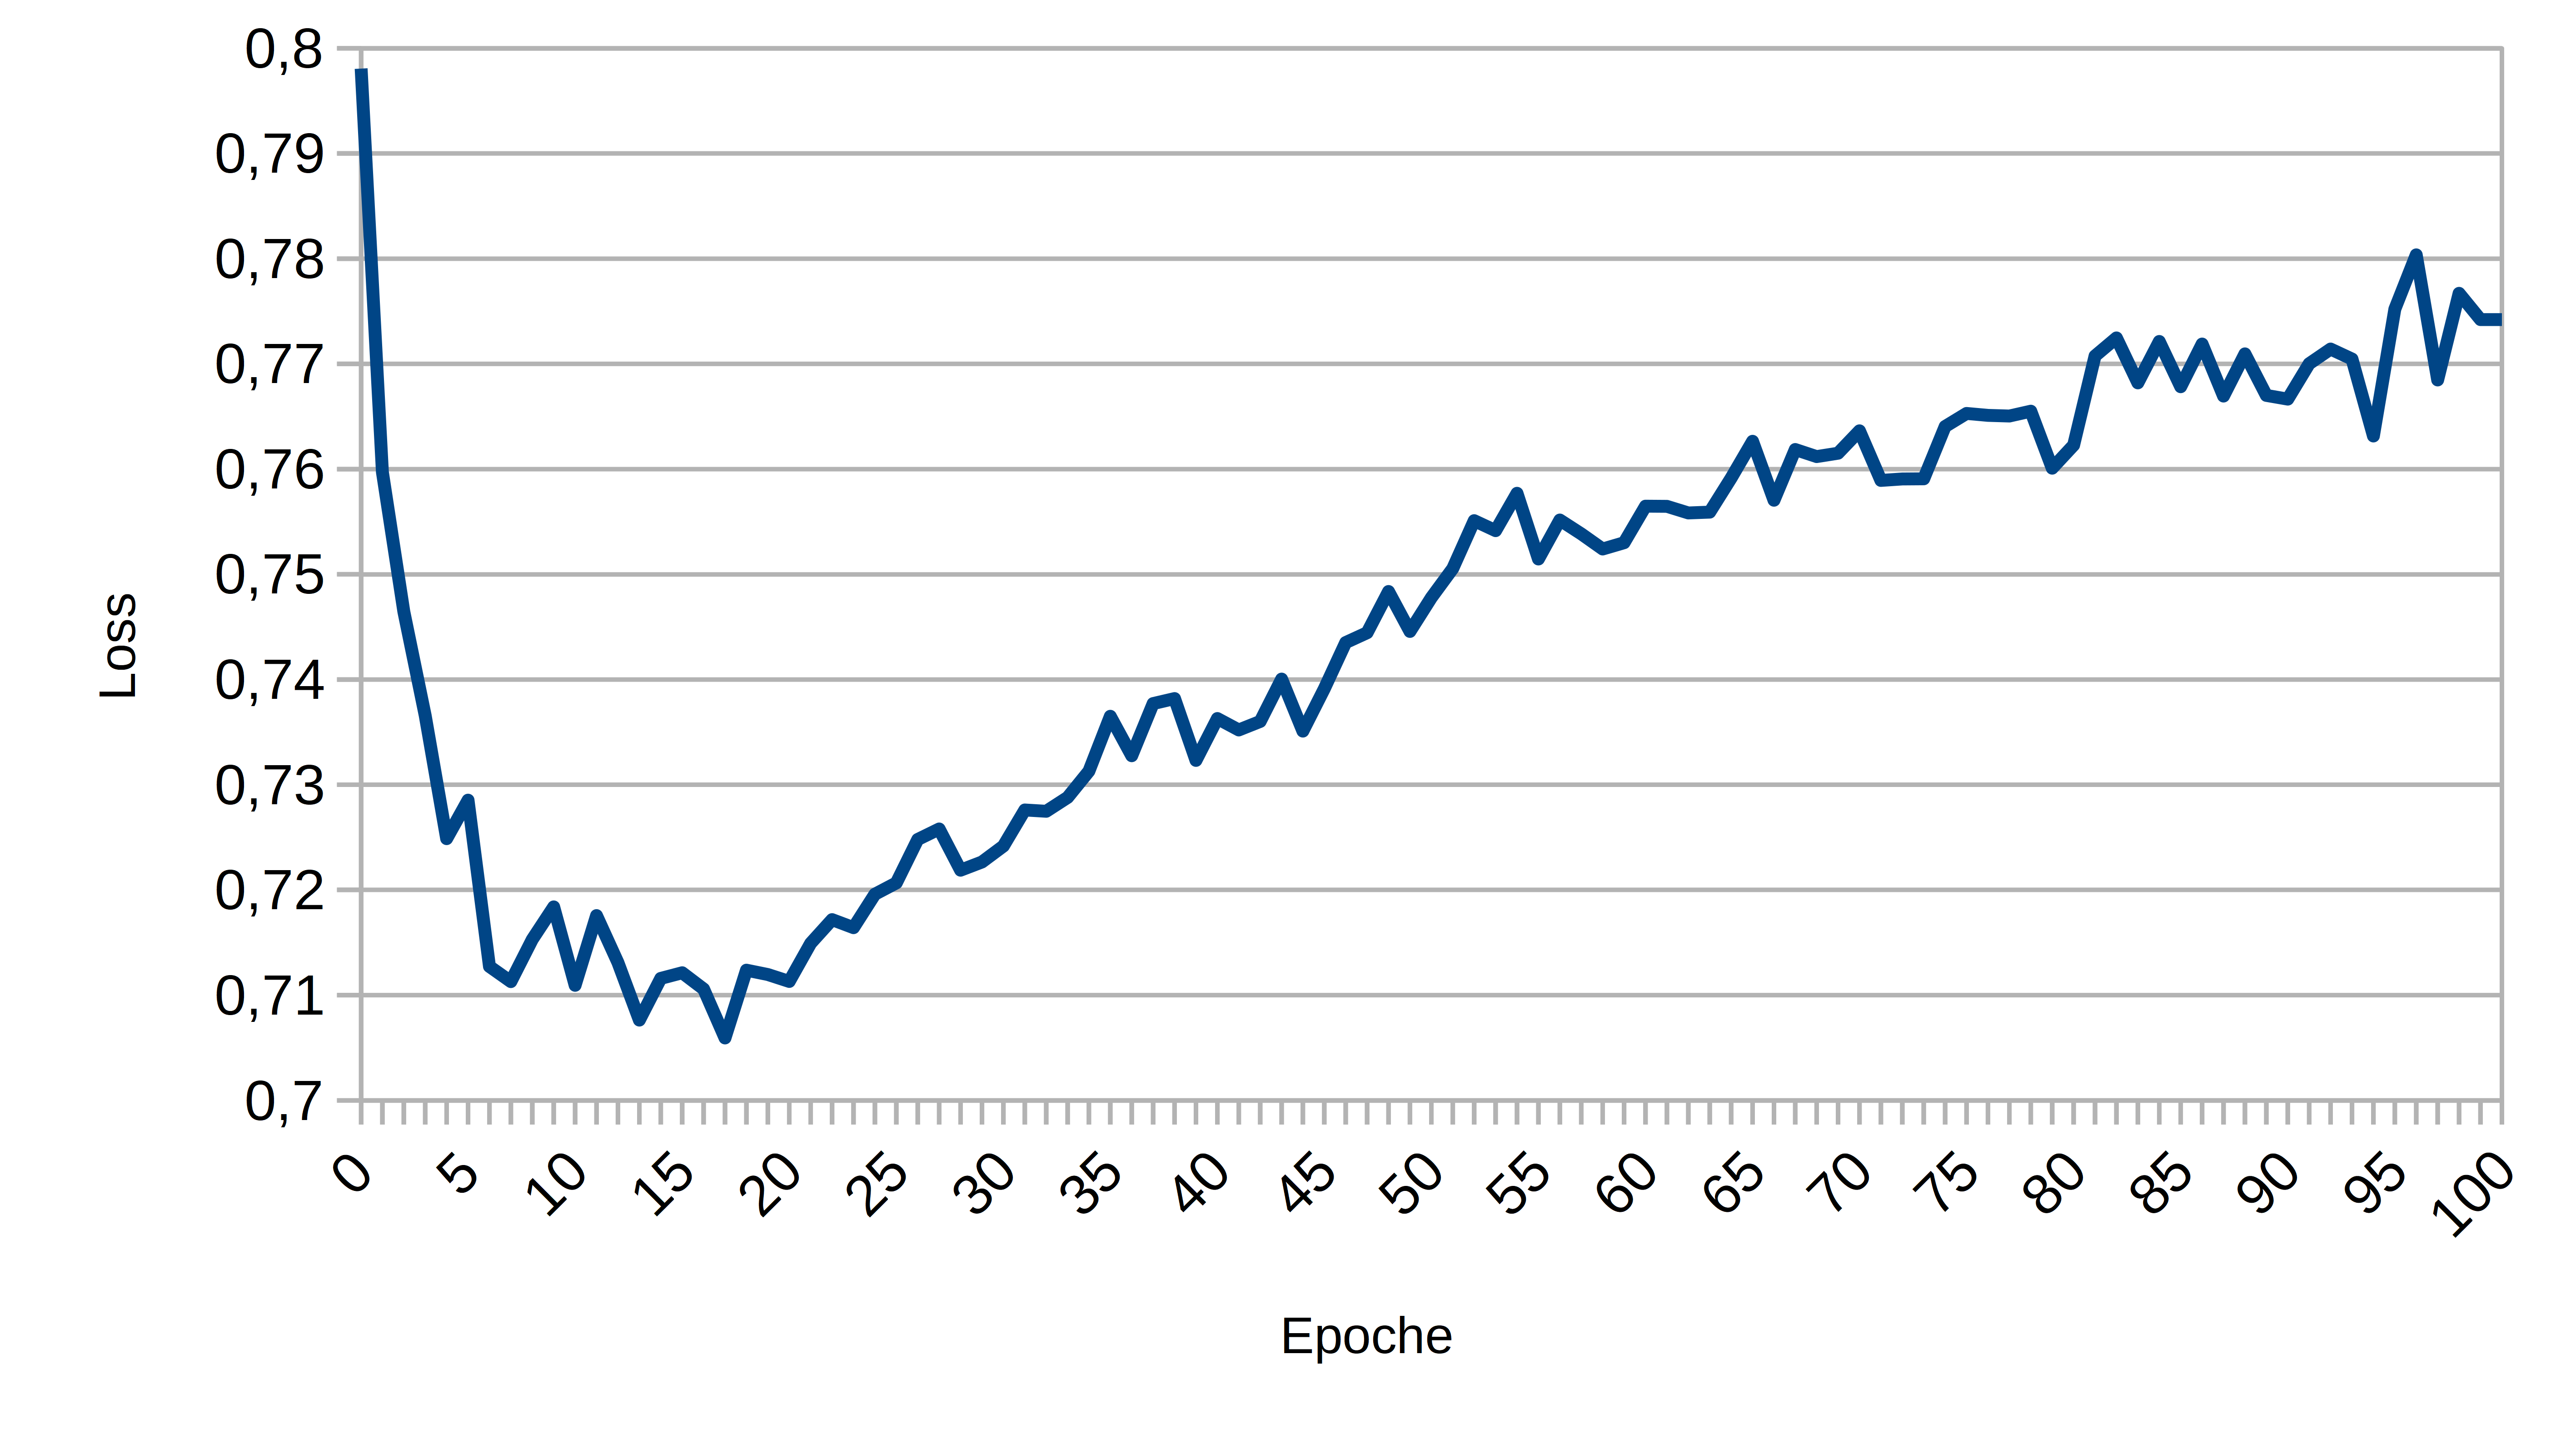
\includegraphics[width=1.0\textwidth]{mlp_5_loss}
	\caption[Overfitting in einem mehrschichtigen Neuronalen Netz]{Nach der 20. Epoche, tritt in diesem mehrschichtigen Neuronalen Netz ein Overfitting auf \cite[S.14]{BA}.}
	\label{fig:mlp_overfitting}
\end{figure}
Zuletzt sei das Underfitting genannt, welches dem Overfitting gegenübersteht. Ein Modell ist dabei zu einfach, um die Strukturen in den Trainingsdaten anzulernen. Modelle mit mehr Parametern, bessere Merkmale oder eine Verringerung der Regularisierung, reduzieren in der Regel ein Overfitting \cite[S.29]{MACHINE_LEARNING}\cite[S.14]{BA}.
\subsubsection{Datenvorverarbeitung für Bilddaten}
Wie im vorherigen Kapitel dargestellt, würden unzureichende Daten zu einer schlechteren Performanz beim Anlernen eines Modells führen. Dies kann auch bei Bilddaten der Fall sein und sollte durch Vorverarbeitungsschritte verhindert werden. In dieser Sektion sollen einige typische Schritte der Bildvorverarbeitung dargestellt werden.
\subsubsection{Qualitätsmaße}
\subsubsection{Testen und Validieren}
\subsection{Neuronale Netze}
\subsection{Konvolutionelle Neuronale Netze}
\section{Datensätze}
\subsection{Sign Language MNIST Dataset}
\subsection{ASL Alphabet Dataset}
\subsection{Videodatensätze}
\section{Entwicklungsprozess}
\subsection{Entwickelte Modelle}
\subsubsection{Neuronale Netze}
\subsubsection{Konvolutionelle Neuronale Netze}
\subsubsection{Transferlearning mittels VGG19}
\subsection{Backend der Webanwendung}
\subsection{Frontend der Webanwendung}
\subsection{Ergebnisse der Entwicklung}
\section{Fazit} 
\section{Ausblick}
\setcounter{biburllcpenalty}{7000}
\setcounter{biburlucpenalty}{8000}
\printbibliography[title=Quellen]
\end{document}